\section{Durchführung}
\label{sec:Durchführung}
Zur Aufnahme der Dampfdruckkurve im Druckbereich $p \leq \SI{1}{\bar}$ kann die Apperatur wie in Abbildung \ref{fig:aufa} aufgebaut werden.
\begin{figure}
    \centering
    \caption{Skizze der Messapperatur im Druckbereich $p\leq \SI{1}{\bar}$.\cite{v203}}
    \label{fig:aufa}
    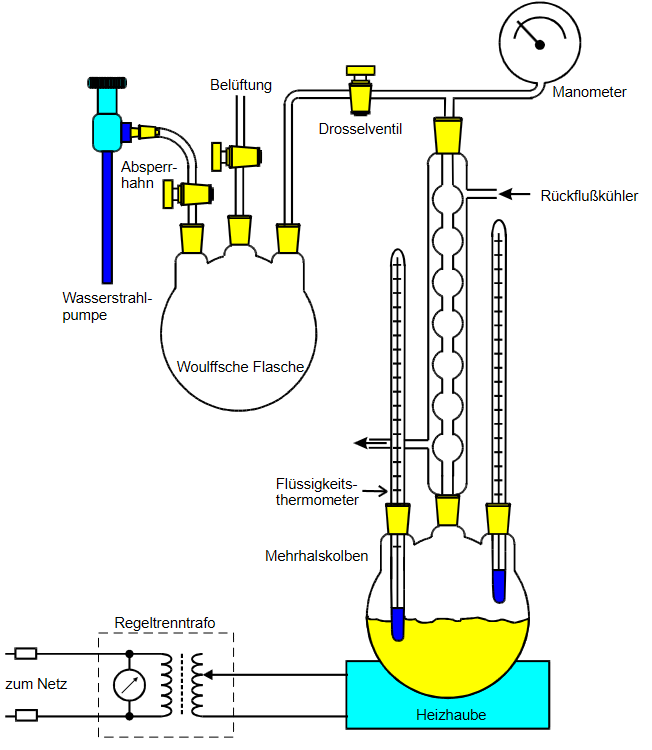
\includegraphics[width = 0.6 \textwidth]{pics/aufbau.png}
\end{figure}
Die Evakuierung erfolgt mit Hilfe einer Wasserstrahlpumpe, wobei der Absperrhahn und das Drosselventil geöffnet werden, während das Belüftungsventil geschlossen wird.
Bis sich ein konstanter Druck einstellt, welcher von der Leitungswassertemperatur abhängt, wird die Wasserstrahlpumpe angestellt.
Das Drosselventil und der Absperrhahn werden geschlossen.
Anschließend wird die Wasserkühlung eingestellt, um die aufsteigenden Dämpfe zu kondensieren. Die Flüssigkeit im Mehrhalskolben wird mit Hilfe der Heizhaube erhitzt.
Sobald sich die Temperatur im Wasser um $\SI{5}{\celsius}$ erhöht hat, wird die Temperatur und der zugehörige Druck am Thermometer im Gasraum beziehungsweise am Manometer abgelesen.
Die Messung wird bis die Wassertemperatur etwa $\SI{90}{\celsius}$ beträgt durchgeführt.
\begin{figure}
    \centering
    \caption{Skizze der Messapperatur im Druckbereich $p \geq \SI{1}{\bar}$.\cite{v203}}
    \label{fig:aufb}
    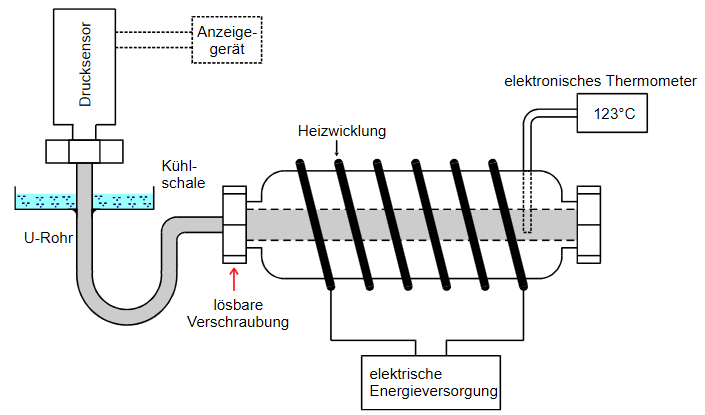
\includegraphics[width = 0.6 \textwidth]{pics/aufbaub.png}
\end{figure}
Für die Hochdruckmessung im Bereich $\SI{1}{\bar}$ bis $\SI{15}{\bar}$ wird die Apperatur verwendet, welche in Abbildung \ref{fig:aufb} zu sehen ist.
Diese ist bereits vor dem Versuch vorbereitet. Es kann sofort die Heizung angestellt werden. Die Datenpaare von Druck und Temperatur werden pro bar notiert. Der Versuch wird durchgeführt bis $\SI{15}{\bar}$ erreicht sind.